\documentclass[jou]{apa6}

\usepackage[american]{babel}

\usepackage{csquotes}
\usepackage[style=apa,sortcites=true,sorting=nyt,backend=biber]{biblatex}
\DeclareLanguageMapping{american}{american-apa}
\addbibresource{bibliography.bib}


%%%%%%%%%%%%%%%%%%%%%%%%%%%%%%%%%%%%%%%%
%% Discrete Structures
%% The start of RBS stuff
%%%%%%%%%%%%%%%%%%%%%%%%%%%%%%%%%%%%%%%%

% Working internal and external links in PDF
\usepackage{hyperref}
% Extra math symbols in LaTeX
\usepackage{amsmath}
\usepackage{gensymb}
\usepackage{amssymb}
% Enumerations with (a), (b), etc.
\usepackage{enumerate}

\let\OLDitemize\itemize
\renewcommand\itemize{\OLDitemize\addtolength{\itemsep}{-6pt}}

\usepackage{etoolbox}
\makeatletter
\preto{\@verbatim}{\topsep=3pt \partopsep=3pt }
\makeatother

% These sizes redefine APA for A4 paper size
\oddsidemargin 0.0in
\evensidemargin 0.0in
\textwidth 6.27in
\headheight 1.0in
\topmargin -24pt
\headheight 12pt
\headsep 12pt
\textheight 9.19in



\title{Sample Quiz 8}
\author{Discrete Structures, Spring 2020}
\affiliation{RBS}

\leftheader{Discrete Quiz 10}

\abstract{%
}

%\keywords{}

\setlength\parindent{0pt}

\begin{document}

\thispagestyle{empty}

\twocolumn
{\Large Discrete Quiz 10}

\vspace{6pt}
{\bf Question 1}\\
Some people participate in an Einkaufshelden program \textendash{} they go 
to one of the shops $A$, $B$ or $C$ and deliver the products to one of the endpoints
$X$, $Y$ or $Z$. Each of the $9$ edges in this full bipartite graph 
$K_{3,3}$ are selected by the same probability. 
\begin{center}
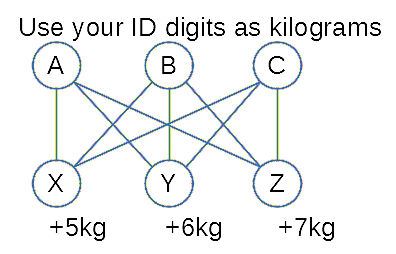
\includegraphics[width=2in]{quiz10.png}
\end{center}
The sum of the numbers on both ends of an edge shows 
how many kilograms of stuff were delivered. (For example, if your Student ID has 
first digit $A=0$, then edge $AZ$ has $0+7 = 7$ kilograms.
Let $X$ denote the random variable: the kilograms of stuff delivered by an Einkaufsheld 
on a single edge.

The variance $V(X)$ can be written as $\frac{m}{n}$, where $m$ and $n$ are relatively 
prime positive integers. Find $m + n$.


\vspace{6pt}
{\bf Question 2.}\\
Given a set of the first positive integers $S = \{ 1,2,\ldots,A+B+(10-C) \}$
(where {\tt A,B,C} are the digits from your student ID:
we define a relation: $aRb$ iff $|a - b| \leq 2$. 

Let $R^2$ be the second power of that relation $R$ and let $M_{R^2}$
be its matrix. Find the number of 1s in this matrix (In other words: 
how many pairs belong to this relation?)


\vspace{6pt}
{\bf Question 3.}\\
Define a set $S$ of these six positive integers: 
\begin{align}
S = \{ & 1+\mathtt{A},\; 2+\mathtt{A}+\mathtt{B},\; 3+\mathtt{A}+\mathtt{B}+\mathtt{C},\;
4 + 2\mathtt{A}+\mathtt{B}+\mathtt{C},\; \nonumber \\
 & 5 + 2\mathtt{A}+2\mathtt{B}+\mathtt{C},\;
6 + 2\mathtt{A}+2\mathtt{B}+2\mathtt{C}\}. \nonumber
\end{align}

Now compute the remainders of the elements of $S$ when divided by $16$. 
You should get another set $S'$ where each element is between $0$ and $15$. 
($S'$ may contain fewer elements than $S$, if some remainders are identical.)
Let $b_i$ be a sequence of bits ($i = 0,\ldots,15$):
$$b_i = 1\;\text{iff}\;i \in S'.$$

We define a matrix for relation $R$ as follows:
$$M_R = \left( \begin{array}{cccc}
b_{0} & b_1 & b_2 & b_3 \\
b_{4} & b_5 & b_6 & b_7 \\
b_{8} & b_9 & b_{10} & b_{11} \\
b_{12} & b_{13} & b_{14} & b_{15} \\
\end{array} \right)$$
Let $M^{\ast}$ be the matrix of the transitive closure of $R$. 
Find the number of 1s in the matrix $M^{\ast}$.


\vspace{6pt}
{\bf Question 4.}\\
Let $S$ be a set and its size is computed from the digits in your ID:
$$|S| = \mathtt{A}+\mathtt{B}+(10 - \mathtt{C}).$$ 
Let $N$ be the number of binary relations on $S$ that are  
reflexive and symmetric at the same time.
Write the last $3$ digits of $N$ in your answer.

{\em Hint} If you need to find the last $3$ digits of some large number, you 
can use periodicity (similar to this: \url{https://bit.ly/33NrJKI}). Euler's theorem 
about the period of remainders modulo $1000$ being periodic with period $\varphi(1000)$ 
(see \url{https://bit.ly/33PyI5Q}) is not directly applicable in this situation,
since your exponent $a$ is not mutually prime with $1000$.
But with some additional reasoning you 
can use Euler's theorem as well.


\vspace{6pt}
{\bf Question 5.}\\
Find the join of the 3-ary relation:
\begin{verbatim}
{ (Wages,MS410,N507),
  (Rosen,CS540,N525),
  (Michaels,CS518,N504),
  (Michaels,MS410,N510) }
\end{verbatim}
and the 4-ary relation:
\begin{verbatim}
{ (MS410,N507,Monday,6:00), 
  (MS410,N507,Wednesday,6:00), 
  (CS540,N525,Monday,7:30),
  (CS518,N504,Tuesday,6:00), 
  (CS518,N504,Thursday,6:00) }
\end{verbatim}
with respect to the last two fields of the first relation and 
the first two fields of the second relation. 

Write the number records in the join.

\vspace{6pt}
{\bf Question 6.}\\
Let $R$ be a relation on $\{a, b, c\}$ that is reflexive and transitive, but not antisymmetric.
Denote its matrix by
$$M_R =  \left( \begin{array}{ccc}
b_{0} & b_1 & b_2 \\
b_{3} & b_4 & b_5 \\
b_{6} & b_7 & b_8 \\
\end{array} \right)$$

Write all the 9 bits (as a sequence of 0s and 1s) in your answer: $b_0b_1b_2b_3b_4b_5b_6b_7b_8$.



\vspace{6pt}
{\bf Question 7.}\\
Let $R$ be a relation on $\{a, b, c\}$ that is reflexive and transitive, but not symmetric.
Denote its matrix by
$$M_R =  \left( \begin{array}{ccc}
b_{0} & b_1 & b_2 \\
b_{3} & b_4 & b_5 \\
b_{6} & b_7 & b_8 \\
\end{array} \right)$$

Write all the 9 bits (as a sequence of 0s and 1s) in your answer.



\end{document}

